\documentclass[11pt]{article}
\usepackage[a4paper,margin=24mm,headheight=15pt,headsep=8mm,footskip=11mm]{geometry}
\usepackage[T1]{fontenc}
\usepackage{lmodern,microtype}
\usepackage{amsmath,amssymb,amsthm,mathtools}
\usepackage{graphicx,booktabs,array,enumitem}
\usepackage{fancyhdr,hyperref}
\hypersetup{colorlinks=false,pdfborder={0 0 0},pdftitle={Komorebi Space: Worked Construction and Proofs},pdfauthor={Operation Komorebi}}
\graphicspath{{figures/}}
\pagestyle{fancy}
\fancyhf{}
\fancyhead[L]{\small\sffamily KOMOREBI SPACE}
\fancyhead[R]{\small\sffamily Worked construction and proofs}
\fancyfoot[L]{\footnotesize\sffamily OPERATION KOMOREBI \quad / \quad VISUAL ATLAS COMPANION v4}
\fancyfoot[R]{\small\thepage}
\renewcommand{\headrulewidth}{0.35pt}
\setlength{\parindent}{0pt}
\setlength{\parskip}{6pt plus 1pt minus 1pt}
\setlength{\emergencystretch}{2em}
\setlist{nosep,leftmargin=*}
\newtheorem{theorem}{Theorem}[section]
\newtheorem{proposition}[theorem]{Proposition}
\newtheorem{lemma}[theorem]{Lemma}
\theoremstyle{definition}
\newtheorem{definition}[theorem]{Definition}
\newtheorem{example}[theorem]{Example}
\theoremstyle{remark}
\newtheorem{remark}[theorem]{Remark}
\newcommand{\R}{\mathbb R}
\newcommand{\Z}{\mathbb Z}
\newcommand{\T}{\mathbb T}
\newcommand{\K}{\mathcal K}
\newcommand{\id}{\mathrm{id}}
\newcommand{\Ext}{\operatorname{Ext}}
\newcommand{\im}{\operatorname{im}}
\newcommand{\Span}{\operatorname{span}}
\newcommand{\norm}[1]{\left\lVert #1\right\rVert}
\newcommand{\ip}[2]{\left\langle #1,#2\right\rangle}
\newcommand{\Cmode}[2]{C_{#1,#2}}
\newcommand{\Smode}[2]{S_{#1,#2}}
\begin{document}
\thispagestyle{empty}
{\small\sffamily O P E R A T I O N\quad K O M O R E B I}\par
\vspace{8mm}
{\Huge\bfseries Komorebi Space}\par
\vspace{2mm}
{\Large Worked construction and proofs}\par
{\large A companion to the multiresolution visual atlas}\par
\vspace{3mm}
{\small 20 October 2026 \quad | \quad Version 4}\par
\vspace{4mm}\hrule\vspace{5mm}

The four surfaces in the atlas are computed graphs of four trigonometric polynomials. They are not four drawings of an unspecified manifold. Their common mathematical object is a compatible tuple of views. This note specifies that tuple, computes its detail and defect coordinates, and proves the identities used to interpret the figures.

The construction is a finite instance of the view and resolution systems in the \emph{Komorebi Space Monograph}, especially Sections 1, 3, 6 and 10 [1]. The Fourier example was introduced for the atlas [2]. The split identity in Section 10 applies here at the level of signal spaces. These signal details are not being identified with that section's particular operator-valued dyadic residual hierarchy.

\begin{quote}
\textbf{Central statement.} The displayed family is an element of a 289-dimensional coherent realization space inside a 404-dimensional raw family space. Its three nonzero detail bands reconstruct its finest view exactly. Its compatibility residual is zero. Altering only view 2 by $\eta=\tfrac15\cos(2\pi u)$ produces the residual $(0,\eta,-\eta)$, which has an exact repair preserving the other three views.
\end{quote}

All of these statements receive ordinary mathematical proofs below. The delivered Python additionally replays the original 8,969 exact checks and passes 3,695 added checks. The resulting 12,664 checks operate on rational Fourier coefficients, including complete bases of the relevant finite spaces. They are not a Lean compiler run and do not replace the infinite-dimensional proof in Section~\ref{sec:infinite}.

\vspace{3mm}
\textbf{Reading route.} Sections 1--4 build the first plate. Section 5 works through the altered family and two different repair objectives. Sections 6--7 explain transport and obstruction. Section 8 identifies the additional hypothesis needed for an infinite family to represent a Hilbert-space element. The two original plates follow the verification record.

\clearpage

\section{Declare the views before drawing them}
\label{sec:views}
The parameter domain is the square torus $\T^2=\R^2/\Z^2$, represented by $0\leq u,v\leq1$ with opposite edges identified. Integrals use normalized area, so $\int_{\T^2}1=1$. Write
\[
 C_{a,b}(u,v)=\cos\bigl(2\pi(au+bv)\bigr),\qquad
 S_{a,b}(u,v)=\sin\bigl(2\pi(au+bv)\bigr).
\]
Choose one representative of each nonzero pair $\{(a,b),(-a,-b)\}$ by requiring $a>0$, or $a=0$ and $b>0$. This avoids duplicating cosine modes or counting a sine mode and its negative as different basis vectors.

For $q\geq1$, let $V_q$ be the real span of the constant function and all such sine and cosine modes with $\max(|a|,|b|)\leq q$. The four views are
\[
 q_n=2^n,\qquad X_n=V_{q_n},\qquad n=0,1,2,3.
\]
These are spaces of functions, not surfaces in three-dimensional Euclidean space. A drawn sheet is the graph of \emph{one} function belonging to one of these spaces.

\begin{lemma}[Orthogonality and dimension]
The displayed real modes form an orthogonal basis of $V_q$. The constant has squared norm 1. Every listed nonconstant sine or cosine has squared norm $1/2$. Consequently
\[
 \dim_{\R}V_q=(2q+1)^2.
\]
\end{lemma}
\begin{proof}
For an integer $m$, integration gives
\[
 \int_0^1 e^{2\pi i mt}\,dt=
 \begin{cases}1&m=0,\\0&m\neq0.\end{cases}
\]
Applying this in both coordinates proves orthogonality of distinct complex characters. Expressing sine and cosine in terms of the two characters at $k$ and $-k$ gives the claimed real inner products. Our representative convention leaves no distinct basis elements with the same pair of frequencies.

There are $(2q+1)^2$ lattice frequencies in the square, including zero. The nonzero ones occur in opposite pairs. Each pair supplies two real basis vectors, so the total is
$1+2((2q+1)^2-1)/2=(2q+1)^2$.
\end{proof}

\begin{center}
\begin{tabular}{@{}cccl@{}}
\toprule
View & Cutoff & Dimension & What is admitted\\
\midrule
$X_0$ & 1 & 9 & Constant and lowest square-frequency modes\\
$X_1$ & 2 & 25 & All preceding modes and the next band\\
$X_2$ & 4 & 81 & All frequencies through square radius 4\\
$X_3$ & 8 & 289 & All frequencies through square radius 8\\
\bottomrule
\end{tabular}
\end{center}

\subsection{The exact functions used in the atlas}
Group the nine nonzero modes in the renderer into four disjoint bands:
\begin{align}
 b_0&=\tfrac12 C_{1,0}+\tfrac3{10}S_{0,1}+\tfrac15 C_{1,1},\label{eq:b0}\\
 d_0&=\tfrac14 S_{2,1}+\tfrac3{20}C_{1,-2},\label{eq:d0}\\
 d_1&=\tfrac18 C_{4,2}+\tfrac1{10}S_{3,-4},\label{eq:d1}\\
 d_2&=\tfrac1{14}S_{8,3}+\tfrac1{16}C_{5,-7}.\label{eq:d2}
\end{align}
The fine seed is $f=b_0+d_0+d_1+d_2\in X_3$. Its views are
\[
 x_0=b_0,\quad x_1=b_0+d_0,\quad
 x_2=b_0+d_0+d_1,\quad x_3=f.
\]
These are the actual coefficients in \texttt{render\_komorebi.py}, not a replacement example chosen after plotting.

At $(u,v)=(0,0)$, all sine terms vanish and all cosine terms equal one. Thus the intermediate values are
\[
 x_0(0,0)=\frac7{10},\quad
 x_1(0,0)=\frac{17}{20},\quad
 x_2(0,0)=\frac{39}{40},\quad
 x_3(0,0)=\frac{83}{80}.
\]
The increments are $3/20$, $1/8$, and $1/16$. These point evaluations illustrate the arithmetic. The proofs below compare full coefficient vectors, not a selection of sample points.

\section{Restrictions, inclusions and compatibility}
Let $\Pi_q$ denote coefficient truncation to square cutoff $q$. On any trigonometric polynomial, it retains precisely the modes satisfying $\max(|a|,|b|)\leq q$. Define
\[
 P_n=\Pi_{q_n}|_{X_{n+1}}:X_{n+1}\longrightarrow X_n,
 \qquad J_n:X_n\hookrightarrow X_{n+1}.
\]
The inclusion $J_n$ leaves the function unchanged and adds zero coefficients at the new frequencies. Restriction is \emph{not} pointwise subtraction or downsampling of the rendered mesh.

\begin{proposition}[Nested projections and sections]
For any two cutoffs $q,r$,
\[
 \Pi_q\Pi_r=\Pi_{\min(q,r)},\qquad \Pi_q^2=\Pi_q,
 \qquad P_nJ_n=\id_{X_n}.
\]
Each $\Pi_q$ is an orthogonal projection for the normalized $L^2$ inner product.
\end{proposition}
\begin{proof}
A basis mode survives two truncations exactly when its frequency lies in both cutoff squares. Their intersection is the smaller square. This proves the first identity on every basis vector and hence on every linear combination. Idempotence is the equal-cutoff case. Every mode in $X_n$ survives the inclusion followed by $P_n$, proving the section identity. The basis is orthogonal, so retaining a subset and deleting its orthogonal complement is an orthogonal projection.
\end{proof}

\begin{proposition}[The plotted family is coherent]
For $n=0,1,2$, $P_nx_{n+1}=x_n$.
\end{proposition}
\begin{proof}
Since $x_n=\Pi_{q_n}f$, nested projections give
\[
 P_nx_{n+1}=\Pi_{q_n}\Pi_{q_{n+1}}f
 =\Pi_{q_n}f=x_n.
\]
For example, $P_1x_2$ deletes the $(4,2)$ and $(3,-4)$ modes in $d_1$ and leaves exactly $x_1$.
\end{proof}

The view category has arrows $i\to j$ for $i\leq j$, while its restriction maps go from $X_j$ to $X_i$. The adjacent restrictions generate the composite ones. Adjacent coherence therefore implies coherence along every arrow of this finite chain.

\section{The realization space, not just the chosen realization}
\label{sec:space}
Put
\[
 E=X_0\oplus X_1\oplus X_2\oplus X_3,\qquad
 R=X_0\oplus X_1\oplus X_2.
\]
Here $R$ records the three \emph{adjacent} defects. The monograph's general arrow-indexed residual has further entries for composite arrows. Those entries are determined here by telescoping the adjacent defects, so this smaller residual space has the same zero set.

Define the linear compatibility operator
\[
 \delta(a_0,a_1,a_2,a_3)=
 (P_0a_1-a_0,\ P_1a_2-a_1,\ P_2a_3-a_2).
\]
The finite Komorebi realization space is
\[
 \K_3=\ker\delta
 =\{a\in E:P_na_{n+1}=a_n\ (n=0,1,2)\}.
\]
A point is the entire compatible tuple. Each of its four components is a view of that point.

\begin{theorem}[Finest-view parameterization]
The map
\[
 \Phi:X_3\longrightarrow\K_3,\qquad
 g\longmapsto(P_0P_1P_2g,\ P_1P_2g,\ P_2g,\ g)
\]
is a linear isomorphism. Its inverse is evaluation at the finest view. In particular,
\[
 \dim E=404,\qquad \dim\K_3=289.
\]
\end{theorem}
\begin{proof}
The tuple $\Phi(g)$ satisfies every adjacent coherence equation by construction. Its finest component is $g$, proving injectivity. Conversely, for a coherent tuple $a$, the three equations imply $a_2=P_2a_3$, $a_1=P_1P_2a_3$, and $a_0=P_0P_1P_2a_3$. Thus $a=\Phi(a_3)$, proving surjectivity and the inverse formula. The dimension of $E$ is $9+25+81+289=404$.
\end{proof}

\begin{theorem}[Exact coherent and defect coordinates]
For $r=(r_0,r_1,r_2)\in R$, define
\[
 Sr=(-r_0-P_0r_1-P_0P_1r_2,\ -r_1-P_1r_2,\ -r_2,\ 0).
\]
Then $\delta S=\id_R$. The operator
\[
 Ca=\Phi(a_3)
\]
satisfies $C^2=C$, $\im C=\K_3$, and
\[
 \boxed{a=Ca+S\delta a.}
\]
Consequently $E\cong\K_3\oplus R$, and $\operatorname{rank}\delta=115$.
\end{theorem}
\begin{proof}
Compute the three entries of $\delta Sr$. The first is
\[
 P_0(-r_1-P_1r_2)-(-r_0-P_0r_1-P_0P_1r_2)=r_0.
\]
The second is $-P_1r_2-(-r_1-P_1r_2)=r_1$, and the third is $0-(-r_2)=r_2$. Hence $\delta S=\id_R$, so $\delta$ is surjective.

The vector $a-S\delta a$ has zero defect and the same finest component as $a$, since $(Sr)_3=0$. The preceding theorem uniquely identifies it as $Ca$. Applying $C$ to an already coherent tuple changes nothing, giving idempotence. The maps
\[
 a\longmapsto(Ca,\delta a),\qquad (k,r)\longmapsto k+Sr
\]
are inverse: $CS=0$, $\delta k=0$, and $\delta S=\id_R$. Finally $\dim R=9+25+81=115$.
\end{proof}

This is a concrete realization of coherent information plus removable defect. The repair $C$ preserves the finest view. It is not generally the orthogonal projection onto $\K_3$ when all four views receive equal weight.

\section{Retained detail and exact reconstruction}
\label{sec:details}
For a coherent family define
\[
 d_n=x_{n+1}-J_nx_n\in X_{n+1}.
\]
\begin{proposition}[The discarded band is retained as a coordinate]
For each $n$, $P_nd_n=0$ and $x_{n+1}=J_nx_n+d_n$. More generally,
\[
 X_{n+1}=J_nX_n\mathbin{\oplus^{\perp}}\ker P_n.
\]
\end{proposition}
\begin{proof}
By coherence and the section identity,
\[
 P_nd_n=P_nx_{n+1}-P_nJ_nx_n=x_n-x_n=0.
\]
The reconstruction equation is the definition rearranged. For arbitrary $z\in X_{n+1}$, use $z=J_nP_nz+(I-J_nP_n)z$. The second summand lies in $\ker P_n$. The two summands have disjoint frequency supports, so the sum is orthogonal and their intersection is zero.
\end{proof}

Substituting the reconstruction equation three times gives the fully typed identity
\[
 x_3=J_2J_1J_0x_0+J_2J_1d_0+J_2d_1+d_2.
\]
Identifying each smaller function space with its inclusion into $X_3$ simplifies this to
\[
 \boxed{x_3=x_0+d_0+d_1+d_2.}
\]
The corresponding coordinate decomposition is
\[
 \K_3\cong X_0\oplus\ker P_0\oplus\ker P_1\oplus\ker P_2,
\]
with dimensions $9+16+56+208=289$. Thus a fixed coarse view $x_0$ leaves 280 real degrees of freedom at the finest level. The nine nonzero modes selected for the illustration form only one particular choice.

\subsection{An exact energy calculation}
Orthogonality of the disjoint bands yields
\[
 \norm{x_3}_2^2=\norm{x_0}_2^2+
 \norm{d_0}_2^2+\norm{d_1}_2^2+\norm{d_2}_2^2.
\]
For example,
\[
 \norm{d_0}_2^2=\frac12\left[\left(\frac14\right)^2+
 \left(\frac3{20}\right)^2\right]=\frac{17}{400}.
\]
The complete arithmetic is
\begin{center}
\begin{tabular}{@{}cll@{}}
\toprule
Component & Calculation & Squared norm\\
\midrule
$x_0$ & $\tfrac12[(1/2)^2+(3/10)^2+(1/5)^2]$ & $19/100$\\[2pt]
$d_0$ & $\tfrac12[(1/4)^2+(3/20)^2]$ & $17/400$\\[2pt]
$d_1$ & $\tfrac12[(1/8)^2+(1/10)^2]$ & $41/3200$\\[2pt]
$d_2$ & $\tfrac12[(1/14)^2+(1/16)^2]$ & $113/25088$\\
\bottomrule
\end{tabular}
\end{center}
Hence the finest energy missing from the two coarsest views is, respectively,
\[
 \norm{x_3-x_0}_2^2=\frac{17}{400}+\frac{41}{3200}+\frac{113}{25088},
 \qquad
 \norm{x_3-x_1}_2^2=\frac{41}{3200}+\frac{113}{25088}.
\]
None of these positive quantities is a compatibility defect. The family remains exactly coherent because restriction deliberately removes these modes.

\section{Change one view and work out the repair}
\label{sec:repair}
The companion plate uses
\[
 \eta=\frac15C_{1,0},\qquad
 y=(x_0,x_1,x_2+\eta,x_3).
\]
The perturbation belongs to $X_0$, so it survives every displayed restriction. Direct substitution gives
\begin{align*}
 (\delta y)_0&=P_0x_1-x_0=0,\\
 (\delta y)_1&=P_1(x_2+\eta)-x_1=\eta,\\
 (\delta y)_2&=P_2x_3-(x_2+\eta)=-\eta.
\end{align*}
Therefore $\delta y=(0,\eta,-\eta)$. One altered view affects both adjacent comparisons, with opposite signs.

\subsection{Repair while preserving views 0, 1 and 3}
The correction
\[
 h=(0,0,-\eta,0)
\]
is invisible on the protected views and satisfies $\delta h=(0,-\eta,\eta)$. Hence
\[
 y+h=x,\qquad \delta(y+h)=0.
\]
This repair is unique with these protected values: preserving view 3 already forces the entire coherent family by the finest-view theorem. Its squared correction cost in the direct-sum norm on $E$ is
\[
 \norm{h}_E^2=\norm{\eta}_2^2=\frac12\left(\frac15\right)^2=\frac1{50}.
\]
The residual energy is instead $\norm{\delta y}_R^2=2\norm{\eta}_2^2=1/25$. These measure different things.

\subsection{The closest repair when no view is protected}
Give all four views equal weight in $\norm{a}_E^2=\sum_n\norm{a_n}_2^2$. For a Fourier basis mode $k$, let
\[
 I_k=\{n:\max(|k_1|,|k_2|)\leq q_n\}.
\]
Coherence requires the coefficient of $k$ to have one common value across the views in $I_k$. If the observed coefficients are $\alpha_{n,k}$, define
\[
 \bar\alpha_k=\frac1{|I_k|}\sum_{n\in I_k}\alpha_{n,k}.
\]
\begin{theorem}[Unconstrained least squares repair]
Replacing each coefficient by its mean over the views in which it occurs gives the unique nearest coherent family.
\end{theorem}
\begin{proof}
Different modes are orthogonal, so the objective separates into independent scalar problems. For one mode, its common basis norm contributes the same positive factor to each view. The identity
\[
 \sum_{n\in I_k}(\alpha_{n,k}-t)^2
 =\sum_{n\in I_k}(\alpha_{n,k}-\bar\alpha_k)^2
  +|I_k|(t-\bar\alpha_k)^2
\]
proves that the unique minimizing common coefficient is $t=\bar\alpha_k$. Combining the finitely many minimizers yields a coherent family and the unique global minimum.
\end{proof}

For the displayed perturbation, the changed low-frequency mode is visible in all four views. Its mean shift is $\eta/4$. Thus
\[
 z=(x_0+\eta/4,\ x_1+\eta/4,\ x_2+\eta/4,\ x_3+\eta/4)
\]
is the unprotected nearest coherent family. Its correction to $y$ is
\[
 z-y=(\eta/4,\eta/4,-3\eta/4,\eta/4),
\]
and
\[
 \norm{z-y}_E^2=\frac{1+1+9+1}{16}\norm{\eta}_2^2
 =\frac3{200}<\frac1{50}.
\]
It is cheaper because it changes the previously protected views. The two answers solve different declared optimization problems. Neither can be substituted silently for the other.

\section{An exact transfer between representations}
Define the coordinate-swap transfer
\[
 (Tf)(u,v)=f(v,u).
\]
It maps $X_n$ to itself because swapping $(a,b)$ to $(b,a)$ preserves the square cutoff. The representative convention may introduce a sine sign. For example,
\[
 T S_{3,-4}=S_{-4,3}=-S_{4,-3}.
\]
\begin{proposition}[Naturality of the swap]
$T^2=I$, $\Pi_qT=T\Pi_q$, and therefore
\[
 P_nT|_{X_{n+1}}=T|_{X_n}P_n.
\]
It follows that $T$ maps coherent families to coherent families and transports their details to the corresponding details.
\end{proposition}
\begin{proof}
Swapping twice restores the original coordinates. A mode is retained by $\Pi_q$ exactly when its swapped frequency is retained, proving commutation on every mode. Linearity gives the operator identity. Thus for a coherent family,
\[
 P_n(Tx_{n+1})=T(P_nx_{n+1})=Tx_n.
\]
The inclusions also commute with $T$, so the new detail is
$Tx_{n+1}-J_nTx_n=T(x_{n+1}-J_nx_n)=Td_n$.
\end{proof}

The cutoff symmetry is a hypothesis, not a stylistic choice. If a truncation retains $|a|\leq1$, $|b|\leq2$, it keeps $C_{0,2}$ but discards its swap $C_{2,0}$. That asymmetric truncation does not commute with $T$. The delivered verifier includes this as a negative control.

\section{A residual is not yet an obstruction}
\label{sec:obstruction}
For a declared linear compatibility map $\delta:E\to R$, let $p_U$ select the values that must remain fixed. Allowed corrections form $N_U=\ker p_U$. The possible changes in residual form $\delta(N_U)$. A raw lift $a$ of prescribed data $s$ therefore defines
\[
 \mathfrak o_U(s)=[\delta a]\in R/\delta(N_U).
\]
For coherent partial sections this is the additive extension obstruction of the monograph [1, Section 3].

\begin{theorem}[Protected extension criterion]
The class does not depend on the chosen raw lift. It vanishes exactly when some coherent family agrees with the prescribed data.
\end{theorem}
\begin{proof}
Two raw lifts differ by an element of $N_U$, so their defects differ by an element of $\delta(N_U)$. This proves independence. The class vanishes precisely when $\delta a=\delta h$ for an allowed $h\in N_U$. Then $a-h$ is coherent and retains the prescribed values. Conversely, any coherent extension $x$ gives $h=a-x\in N_U$ and $\delta h=\delta a$.
\end{proof}

For the altered Fourier family, protection of views $0,1,3$ permits changes only at view 2. Such changes have the form
\[
 h=(0,0,k,0),\qquad \delta h=(0,P_1k,-k).
\]
On the adjacent residual space the quotient can be represented explicitly by
\[
 \Omega(r_0,r_1,r_2)=(r_0,\ r_1+P_1r_2)\in X_0\oplus X_1.
\]
Indeed $\Omega$ is surjective, and $\ker\Omega=\delta(N_U)$: if $r_0=0$ and $r_1=-P_1r_2$, choose $k=-r_2$. Thus this quotient has dimension $9+25=34$, but the displayed residual has zero class:
\[
 \Omega(0,\eta,-\eta)=(0,0).
\]
The nonzero defect is entirely removable by an allowed change.

\subsection{Why this chain does not exhibit a genuine extension obstruction}
Every internally coherent partial section of this finite split tower extends. To prove this, let $m$ be its largest prescribed index. Include the value at $m$ into $X_3$ by adding zero higher coefficients, then restrict to all lower views. Coherence on the prescribed full subcategory ensures the required lower values are recovered. If no views are prescribed, the zero family is an extension.

Thus this specific chain is an excellent model of views, retained detail and repair, but not of a nonzero obstruction for internally coherent partial data. Fixing inconsistent values at two comparable levels would not supply such an example: those values would already fail to form a coherent partial section.

\subsection{A small branching model with a nonzero obstruction}
Use the view category $a\to w\leftarrow b$ and real fibers. Its restriction maps are
\[
 \rho_a(t)=t,\qquad \rho_b(t)=2t.
\]
A coherent full family has the form $(x_a,x_w,x_b)=(t,t,2t)$. Prescribe the two endpoint views $U=\{a,b\}$ with values $(1,3)$. This is internally coherent because there is no nonidentity arrow between the two endpoints.

A raw lift is $(1,t,3)$ and its defect is $(t-1,2t-3)$. Corrections preserving both endpoints change only $t$ and produce defects $(h,2h)$. The quotient map
\[
 \omega(r_a,r_b)=2r_a-r_b
\]
has kernel exactly $\{(h,2h):h\in\R\}$. Therefore
\[
 \mathfrak o_U(1,3)\ \widehat{=}\ 2(t-1)-(2t-3)=1\neq0.
\]
No choice of the middle value repairs the two protected observations. This branching example, unlike the altered Fourier tuple, demonstrates a genuine nonzero extension obstruction.

\section{What changes for infinitely many resolutions?}
\label{sec:infinite}
Now let $X_n=V_{2^n}$ for every $n\geq0$. Let $H$ be the Hilbert completion of the union of these spaces under the normalized $L^2$ norm. Defining $H$ this way supplies exactly the completeness and density used below, without importing a separate Fourier completeness theorem.

The algebraic realization space consists of all sequences $(x_n)$ satisfying $P_nx_{n+1}=x_n$. This definition by itself imposes no uniform norm bound.

\begin{theorem}[A finite energy budget is exactly the missing condition]
For a coherent infinite family, the following are equivalent:
\begin{enumerate}[label=(\roman*)]
\item There is a unique $f\in H$ with $\Pi_{2^n}f=x_n$ for every $n$.
\item $\sup_n\norm{x_n}_2<\infty$.
\item $\norm{x_0}_2^2+\sum_{n\geq0}\norm{d_n}_2^2<\infty$, where $d_n=x_{n+1}-J_nx_n$.
\end{enumerate}
When these hold, $x_n\to f$ in norm and
\[
 \norm{f}_2^2=\norm{x_0}_2^2+\sum_{n\geq0}\norm{d_n}_2^2,
 \qquad
 \norm{f-x_n}_2^2=\sum_{j\geq n}\norm{d_j}_2^2.
\]
\end{theorem}
\begin{proof}
The finite orthogonal decomposition gives
\[
 \norm{x_n}_2^2=\norm{x_0}_2^2+\sum_{j<n}\norm{d_j}_2^2,
\]
so (ii) and (iii) are equivalent. If (i) holds, projection is contractive, giving $\norm{x_n}_2\leq\norm{f}_2$ and hence (ii).

Assume (ii). For $m\geq n$, coherence says $\Pi_{2^n}x_m=x_n$, so $x_m-x_n$ is orthogonal to $x_n$. Consequently
\[
 \norm{x_m-x_n}_2^2=\norm{x_m}_2^2-\norm{x_n}_2^2.
\]
The squared norms are increasing and bounded. They converge, making $(x_n)$ Cauchy. Completeness supplies $f\in H$. Each finite projection is a bounded operator and hence extends continuously to $H$. Passing to the limit in $\Pi_{2^n}x_m=x_n$ gives $\Pi_{2^n}f=x_n$.

If $f$ and $g$ have the same projections, $f-g$ is orthogonal to every $X_n$, hence to their dense union, and therefore equals zero. This proves uniqueness. Taking limits in the finite energy identities proves both remaining formulas.
\end{proof}

\begin{example}[Perfect finite coherence without a Hilbert realization]
Set
\[
 w_n(u,v)=\sum_{k=1}^{2^n}\cos(2\pi k u).
\]
Every adjacent restriction satisfies $P_nw_{n+1}=w_n$. Yet orthogonality gives
\[
 \norm{w_n}_2^2=\frac{2^n}{2}=2^{n-1}\longrightarrow\infty.
\]
Thus $(w_n)$ is an algebraically coherent point but is not the projection family of an element of $H$.
\end{example}

The displayed nine-mode seed has a Hilbert realization: retain that same polynomial at all finer levels and set every additional detail to zero. It is only one possible continuation of the first four views. Those four views alone do not determine unknown higher-frequency coefficients. Uniqueness in the theorem concerns an entire infinite coherent family satisfying the norm condition.

\section{Verification record and provenance}
The following checks were actually executed for this edition:
\begin{center}
\begin{tabular}{@{}lr@{}}
\toprule
Verification group & Passing exact checks\\
\midrule
Original visual-atlas verifier, replayed & 8,969\\
Additional worked-example verifier & 3,695\\
\midrule
Total & 12,664\\
\bottomrule
\end{tabular}
\end{center}
The original verifier tests projector identities, nesting, split reconstruction and coordinate-swap transport on all 289 basis vectors of $X_3$. The added verifier checks every basis vector of the 404-dimensional raw family space and the 115-dimensional adjacent residual space. It verifies both repairs, the right inverse, explicit obstruction coordinates, energies and point calculations. All 81 basis directions of a view-2-only correction are also checked.

Negative controls detect an omitted detail, an incorrect residual sign, confusion between pointwise difference and defect, and a cutoff that breaks coordinate-swap compatibility. The branching obstruction is evaluated at several raw lifts. Its independence from every lift is proved in Section~\ref{sec:obstruction}.

Coefficient arithmetic uses Python's \texttt{Fraction}. Complete basis verification covers the stated linear identities over the real numbers because the operators are linear and have the tested rational matrices. Orthogonality is justified by the written proof. Trigonometric values and page geometry used for drawing remain floating-point calculations. No Lean compilation was performed. The infinite theorem is a written proof, not a consequence of a finite check count.

\subsection*{Reproduction}
From the delivered directory, run
\begin{verbatim}
python verify_worked_example.py --output .
python render_komorebi.py --output figures --dpi 300
\end{verbatim}
The first command writes the verification and intermediate-step JSON records. The second recreates the plates. NumPy and Matplotlib must already be installed for offline use. Rebuild this PDF with two runs of \texttt{pdflatex} on the delivered source.

\subsection*{Sources}
\begingroup\small
\textbf{[1]} \emph{Komorebi Space Monograph v1.13.0}, Sections 1, 3, 6 and 10: coherent realization, additive obstruction, exact tower transport, split reconstruction and convergence.

\textbf{[2]} \emph{Komorebi Space Visual Atlas v3}. The original renderer and its two plates. The seed, cutoffs, perturbation and plotting conventions are unchanged.

\textbf{[3]} \emph{Worked-example audit v4}. The delivered verifier, \texttt{verification.json} and \texttt{worked\_steps.json}: complete finite basis checks, intermediate coefficients and exact scalar calculations.
\endgroup

\clearpage
\section*{Plate 1\quad One realization at four resolutions}
\addcontentsline{toc}{section}{Plate 1: One realization at four resolutions}
\begin{center}
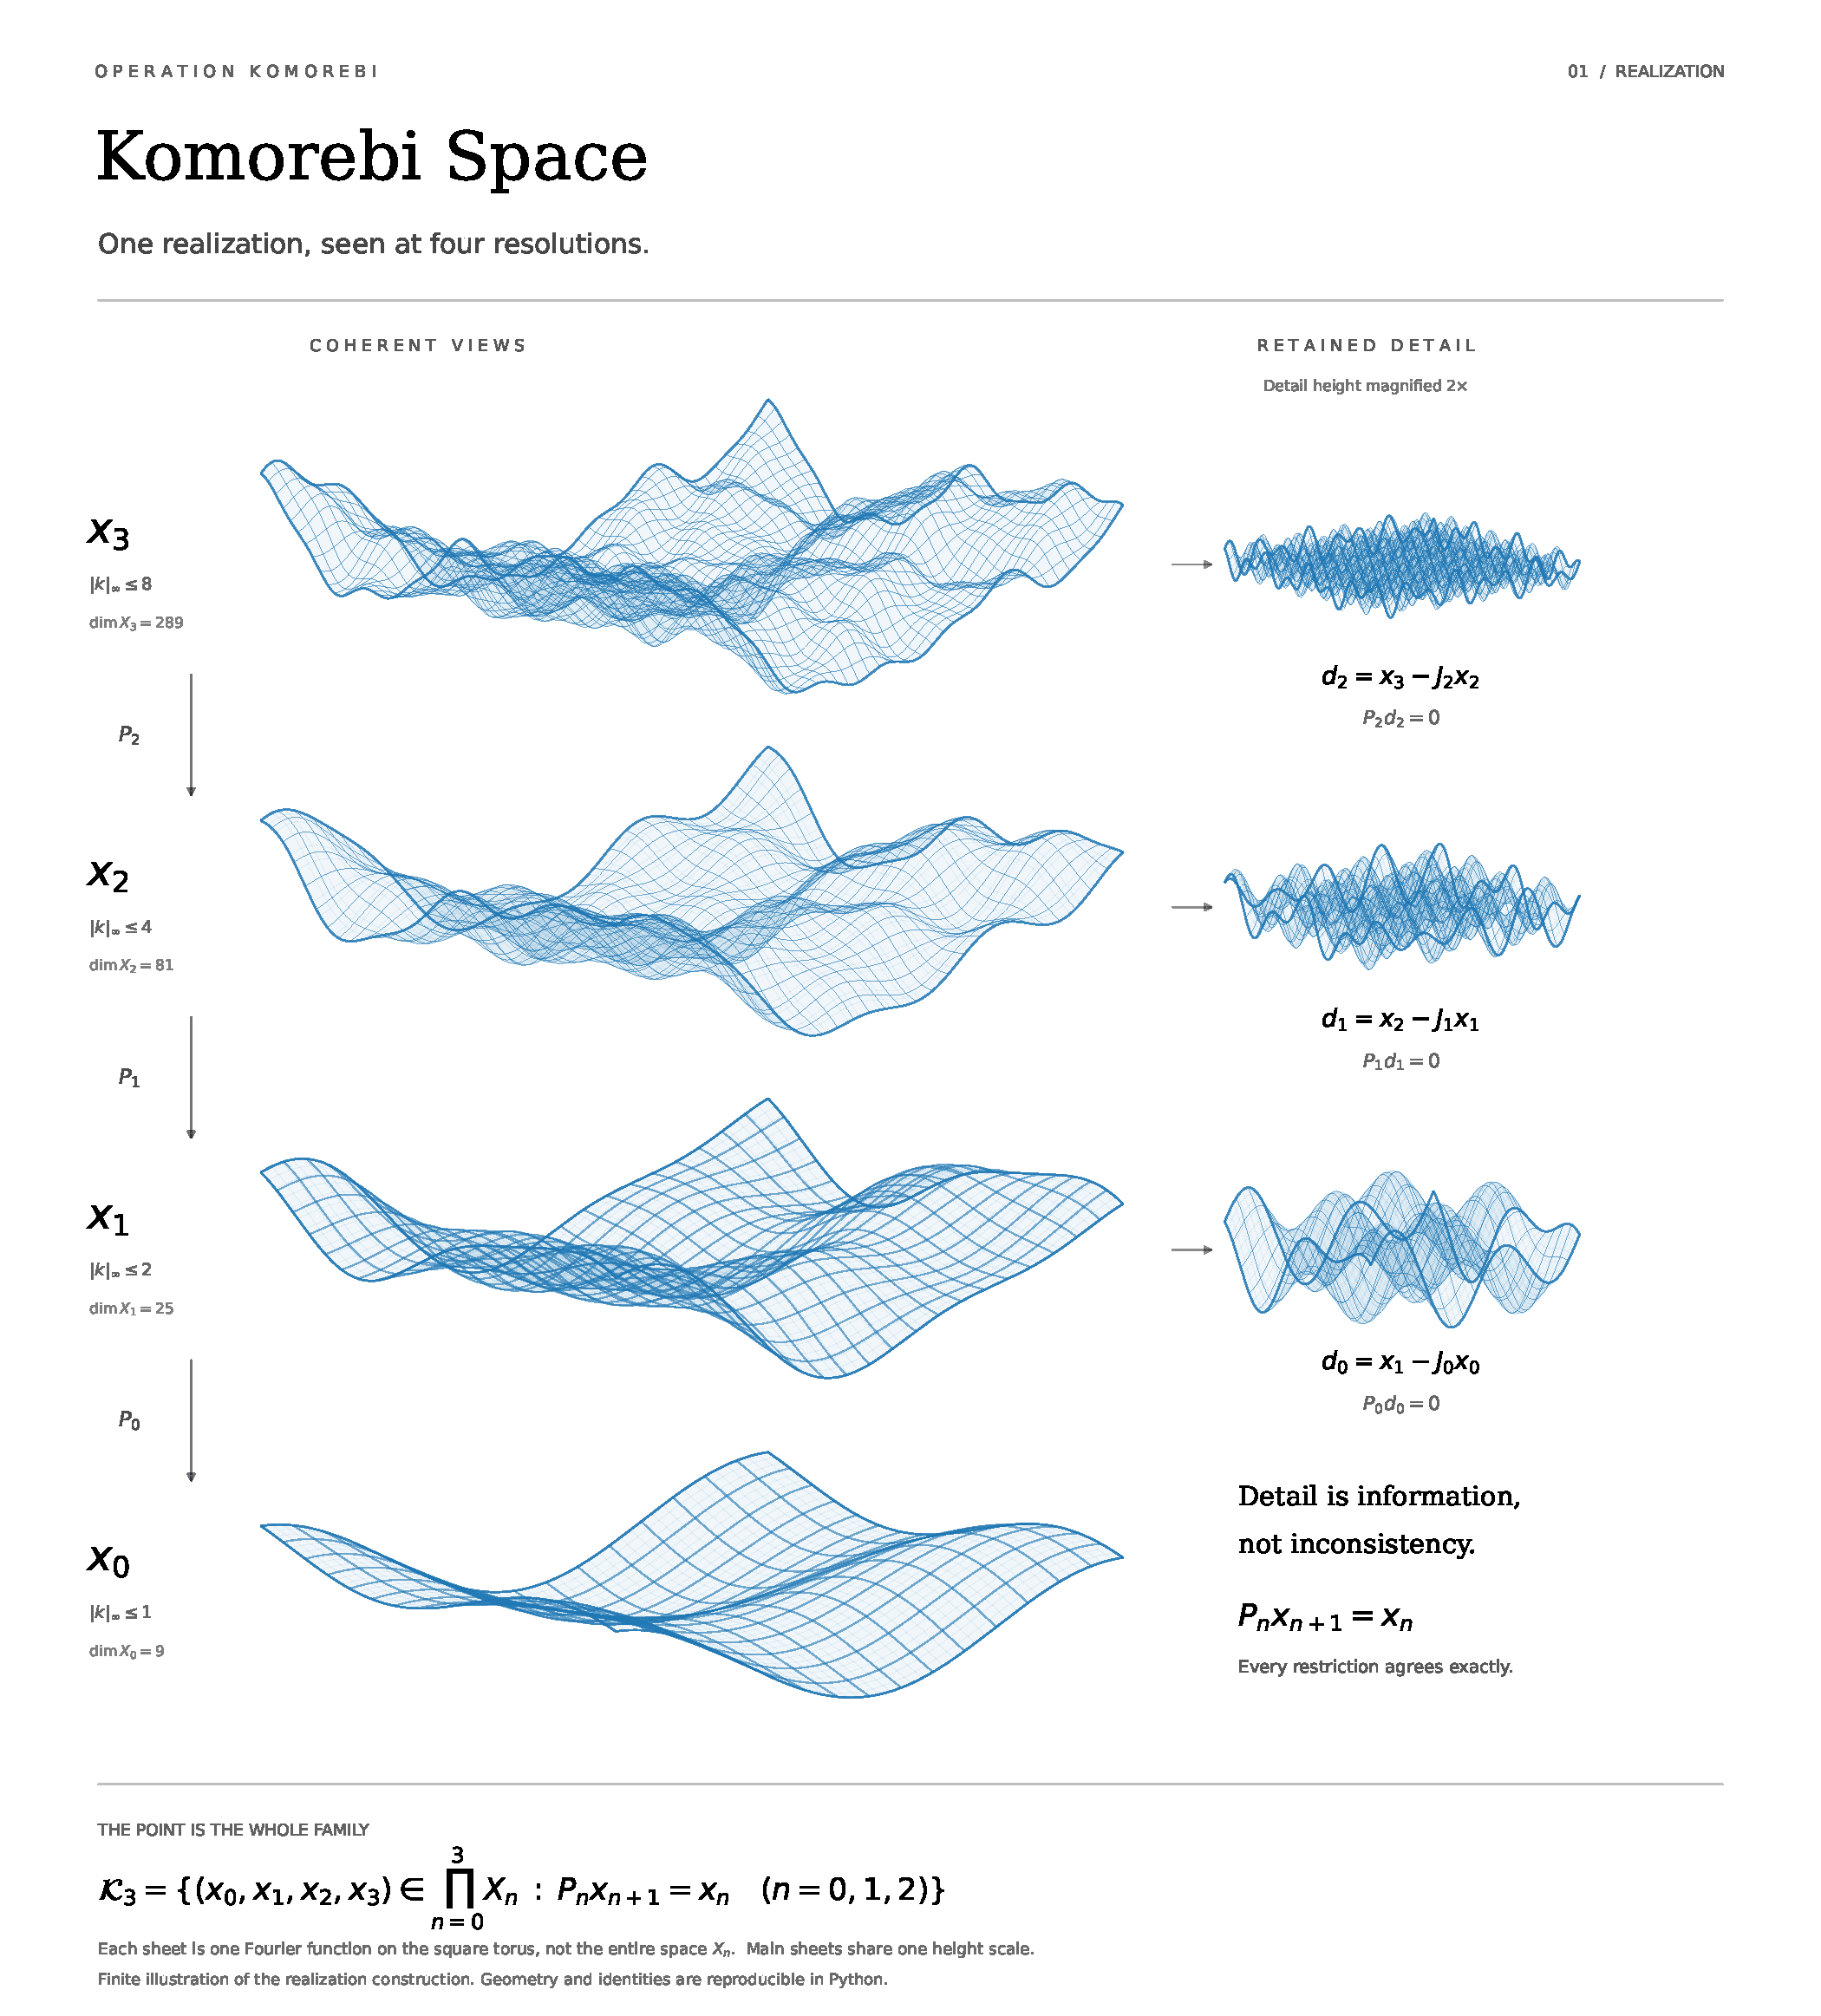
\includegraphics[width=\textwidth,height=0.83\textheight,keepaspectratio]{komorebi_space_resolution.pdf}
\end{center}
{\small Main sheets are graphs of $x_0,x_1,x_2,x_3$ from Section~\ref{sec:views}. Small sheets show the details from Section~\ref{sec:details} with twice the main vertical gain. Their placement separates the views for reading. It adds no mathematical coordinate to $\K_3$.}

\clearpage
\section*{Plate 2\quad Detail, defect and exact repair}
\addcontentsline{toc}{section}{Plate 2: Detail, defect and exact repair}
\begin{center}
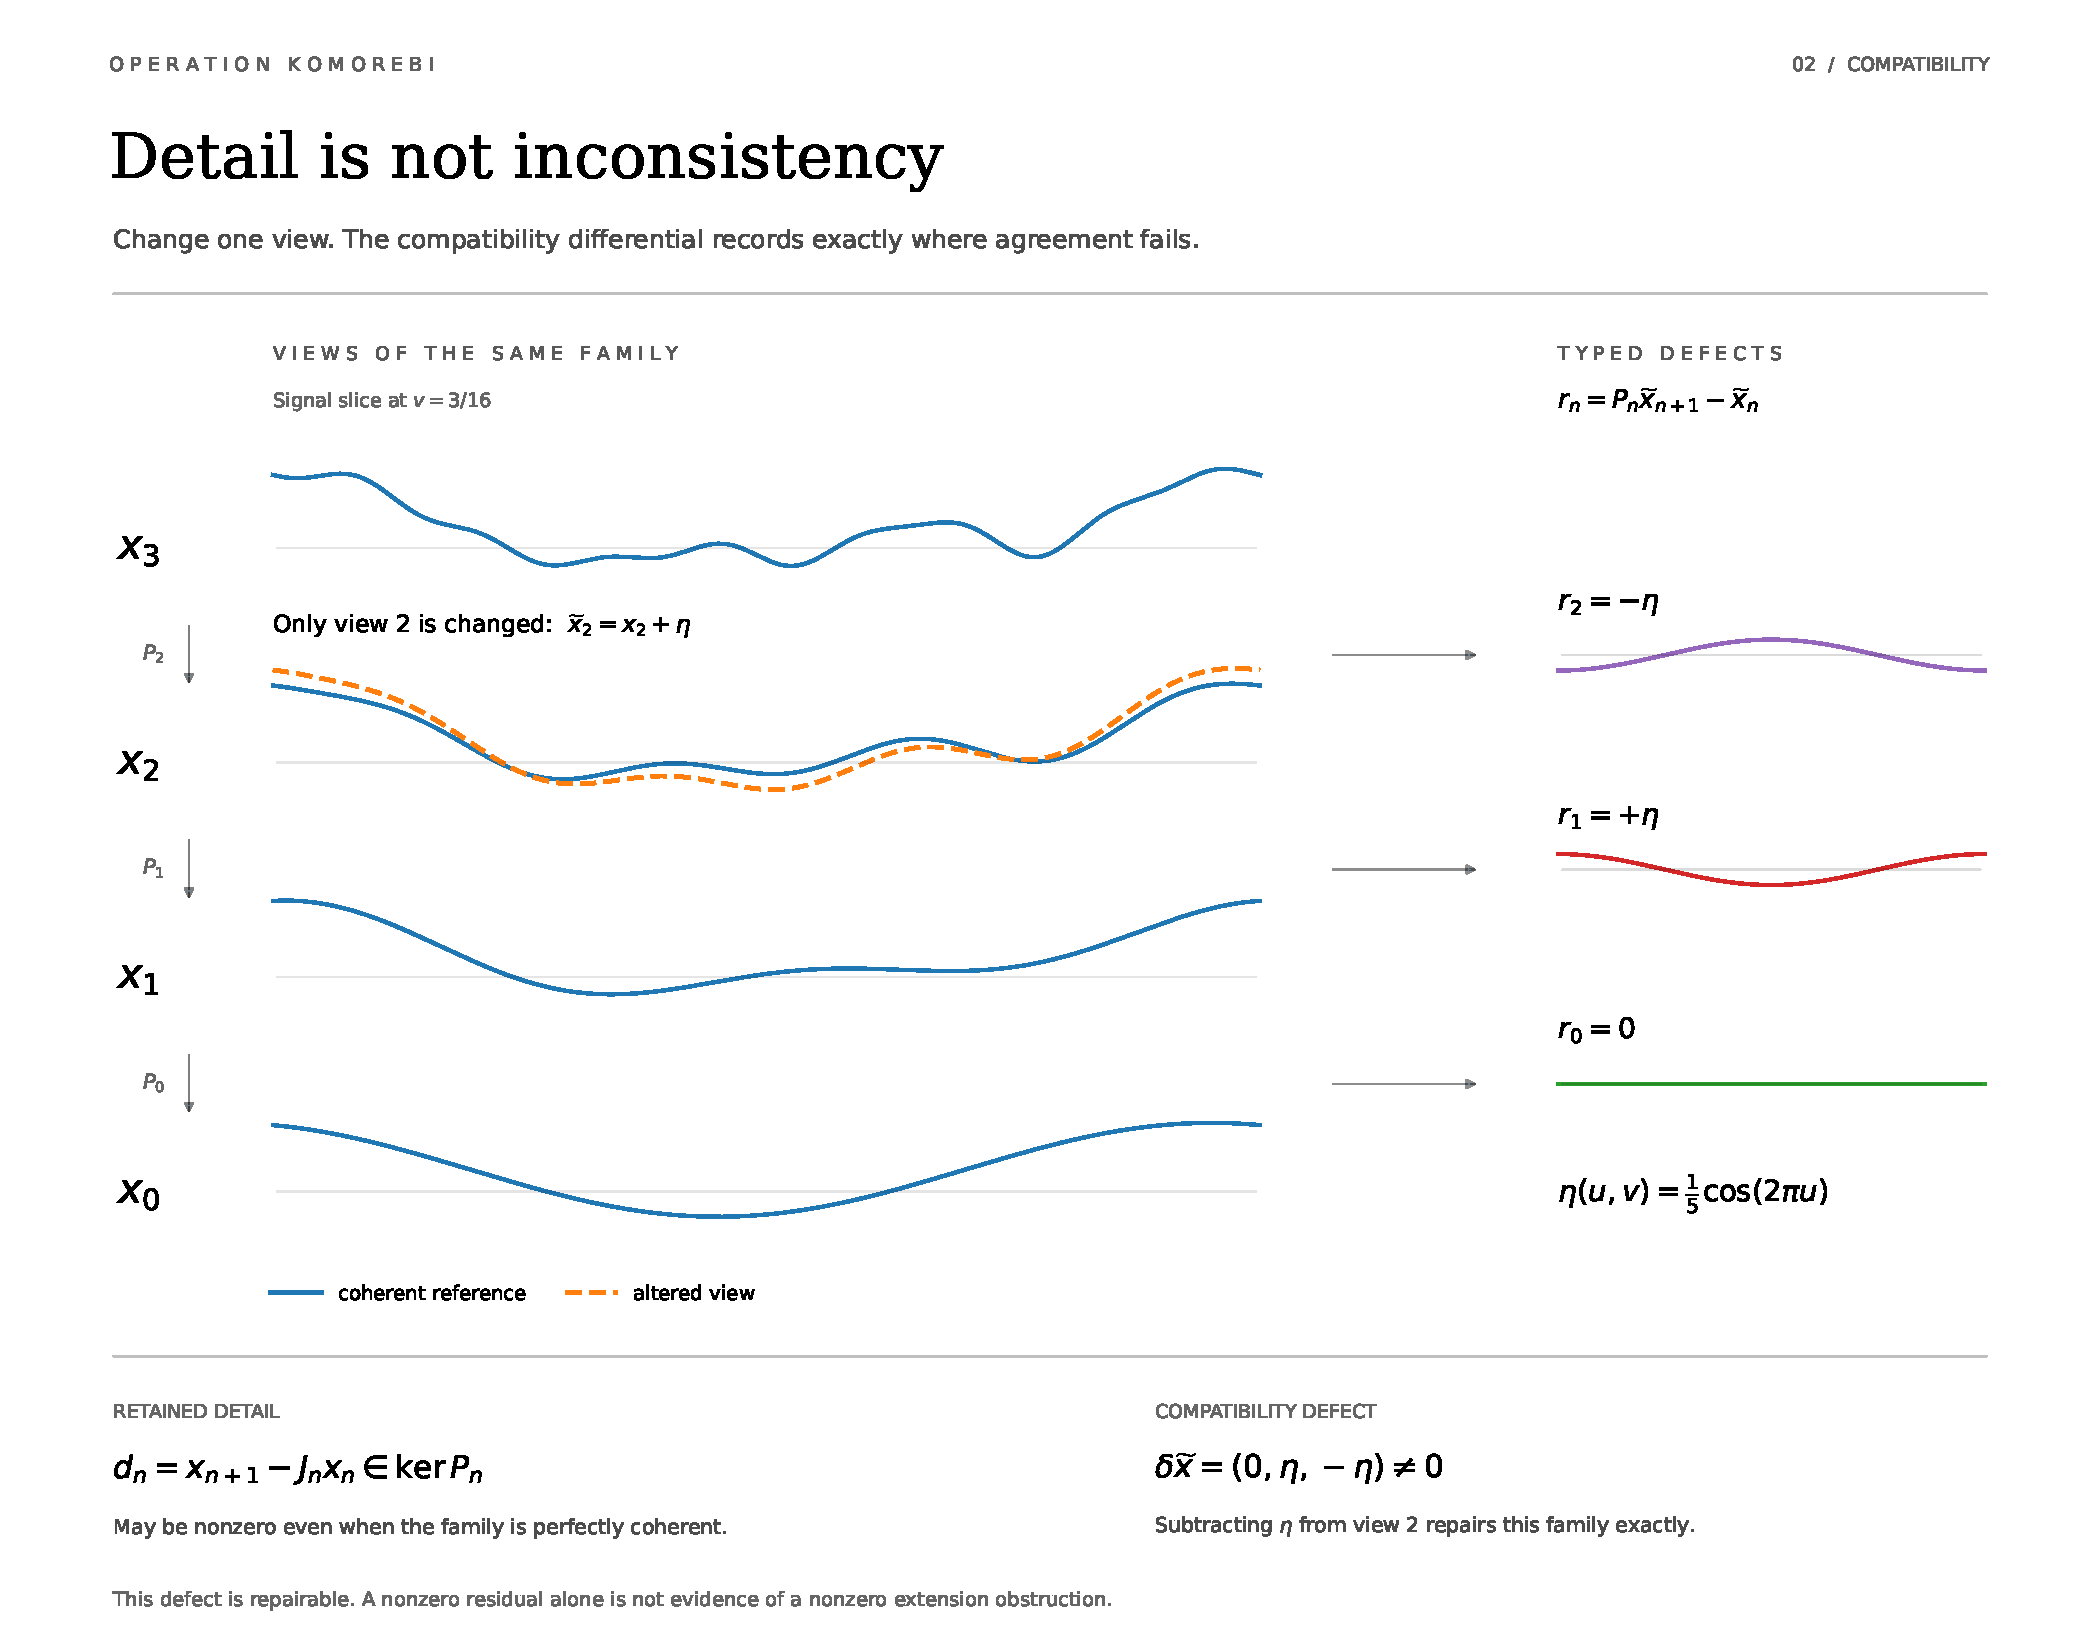
\includegraphics[width=\textwidth,height=0.76\textheight,keepaspectratio]{komorebi_space_compatibility.pdf}
\end{center}
{\small The curves are the slice $v=3/16$ of the exact family and the altered view. The right-hand curves show the typed adjacent defects, with the same vertical gain as the signal curves. Section~\ref{sec:repair} proves their signs and the protected repair. Section~\ref{sec:obstruction} proves why this nonzero residual still has zero protected extension obstruction.}

\vspace{8mm}
\begin{quote}
\textbf{The distinction to retain.} Detail records what a lower resolution cannot see. Defect records disagreement between resolutions. Obstruction records whether the disagreement can be removed without changing the prescribed information.
\end{quote}
\end{document}
